% Dr. Nam H. Le. drnamlabs.com, bunnyquant.com
\documentclass[11pt]{article}

\usepackage[margin=1in]{geometry}
\usepackage[utf8]{inputenc}
\usepackage[T1]{fontenc}
\usepackage{times}
\usepackage{graphicx}
\usepackage{booktabs}
\usepackage{amsmath,amssymb}
\usepackage{xcolor}
\usepackage{caption}
\usepackage{microtype}
\usepackage[numbers,sort&compress]{natbib}
\usepackage[colorlinks=true,allcolors=blue!55!black]{hyperref}

\graphicspath{{../figs/}}
\captionsetup{font=small,labelfont=bf}
\setlength{\parskip}{0.35em}

\newcommand{\goal}[1]{\textit{``#1''}}

\title{\textbf{Most of It Was Toxicity}\\[0.3em]
\large Goal-Conditioned Intervention Retrieval from a Cell Painting Archive,
and the Baselines It Has to Be Scored Against}

\author{Nam H. Le\\
Department of Computer Science, University of Vermont\\
Burlington, VT, USA\\
\texttt{nam.le@uvm.edu}}

\date{\today}

\begin{document}
\maketitle

\begin{abstract}
\noindent
Large archives of perturbation experiments are indexed by what was done to the cells:
a compound name, a gene, a condition. They are not indexed by what the cells ended up
looking like, so a new question asked of an old archive usually means a new screen.
We ask whether such an archive can be addressed by \emph{outcome}, stated in ordinary
English, and answer with an intervention and a dose. Using RxRx3-core, a public Cell
Painting archive of 1{,}671 compounds at eight doses in human endothelial cells, we
learn a map from a sentence describing a desired cellular appearance to a
dose-response curve over every compound in the library, together with a calibrated
decision to refuse when the archive contains nothing that matches.
Our central result is negative and, we argue, more useful than the positive one. Under
the literal reading of per-cell CellProfiler features, the system reaches AUC
$0.842/0.873$ on compounds whose chemical scaffold it has never seen, which looks
strong until the same predictions are scored by a baseline that never reads the
question: taking the model's own prediction for \goal{kill most of the cells} and
using that single vector for every other goal reaches $0.833/0.855$. The
behaviour-specific contribution is $+0.010$/$+0.018$ AUC. The cause is in the
measurement, not the model. CellProfiler averages over segmented survivors, and dying
cells round up and read brighter per unit area, so between 64\% and 69\% of wells
satisfying a per-cell \goal{brighter} predicate have also lost their cells, against a
3.5\% base rate. Redefining every per-cell predicate as ``\emph{X} and the cells were
not killed'' lowers the headline to $0.799/0.861$ and raises the margin over that
baseline tenfold, to $+0.104$/$+0.072$. Scored the way a screening group would score it,
with a budget of eight wells the system finds a real hit for 42\% of held-out goals
against 20\% for the toxicity baseline (paired difference $+22\%$, 95\% CI
$[+11\%,+33\%]$, McNemar $p=0.0005$), while between 16 and 96 wells the two are not
separable. Thirty-eight of the 64 held-out goals are conjunctions whose concept was
never trained. We release the code, the evaluation protocol with its trivial baselines
printed beside every number, and a pre-registered 480-well prospective test that would
settle the claim.
\end{abstract}

\section{Introduction}

A phenotypic screen produces two things: a decision about the compounds that were
tested, and an archive. The decision is used; the archive is usually not, because it
is indexed by treatment. If a screen was run to find compounds that killed a cancer
line, the images it produced also contain every other morphological consequence of
those compounds, and nobody can retrieve them, because the question ``which of these
made the mitochondria dimmer without killing anything'' was never asked and therefore
never labelled.

This paper asks whether the archive can be turned around and addressed by outcome. The
interface is a sentence. The output is a ranked list of (compound, dose) pairs, a
predicted dose-response curve for each, and, when nothing in the archive produces the
requested appearance, a refusal.

Three features of the problem shape everything that follows.

\textbf{There are no labels.} Nobody annotated these wells with ``the mitochondria are
dimmer and the cells are alive''. Supervision has to be manufactured from measurements
that were made for other reasons, which makes the \emph{definition} of each predicate a
modelling decision with consequences, not a formality. Section~\ref{sec:confound} shows
that getting this definition wrong inflates every downstream number by an amount larger
than the entire effect being reported.

\textbf{The right answer includes a dose.} An intervention is not a class label. Many
compounds produce a requested morphology only in a window, because the dose that
produces it strongly also kills, so the output must be able to rise and then fall.

\textbf{A system that always answers is not usable.} A screening group asking for an
effect no compound in the library produces needs to be told so. Refusal is therefore
scored as a first-class output, not described as future work.

\paragraph{Contributions.}
\begin{enumerate}\itemsep0.2em
\item \textbf{A confound in per-cell morphological features, and a protocol that
exposes it} (Section~\ref{sec:confound}). Per-cell intensity features computed over
segmented survivors are strongly entangled with cell death. We quantify the
entanglement, show that it accounts for almost all of the apparent skill of a
language-conditioned model under the literal predicate definition, and give the
redefinition that removes it. The detection protocol, scoring every result against the
model's own toxicity prediction, is cheap and transfers to any work on these archives.
\item \textbf{Goal-conditioned intervention retrieval with dose windows and calibrated
refusal} (Sections~\ref{sec:model}--\ref{sec:results}). A frozen sentence encoder, a
small network trained from scratch, and an explicit non-monotone dose response; refusal
AUC $0.85$ on goals the archive cannot satisfy, using a pool-size-invariant confidence
statistic.
\item \textbf{Evaluation in screening cost, not only in AUC}
(Section~\ref{sec:screening}). Given a budget of $k$ wells, how often does the shortlist
contain something that actually does what was asked? Reported against two trivial
baselines and random order, including the budgets at which the trivial baselines win.
\item \textbf{A negative result on vision-language models as a label source}
(Section~\ref{sec:vlm}), measured against the physical measurements behaviour by
behaviour on 2{,}000 blind-scored groups.
\item \textbf{A pre-registered prospective test} (Section~\ref{sec:prereg}) that would
convert a retrospective method into a validated instrument for roughly 480 wells.
\end{enumerate}

\section{Related work}

\paragraph{Language and morphological profiling.}
CellCLIP~\citep{lu2025cellclip} and MorphoCLIP~\citep{ilyosbekov2026morphoclip} align
Cell Painting images with text that \emph{describes the perturbation that was applied},
contrastively, and retrieve in that space. The direction is forward: given a treatment,
find its images, or given images, name the treatment. The present work runs the other
way, from a desired outcome to the intervention and its dose, which changes the
supervision problem (there is no text to align with, because the desired outcome was
never recorded) and the output type (a dose-response curve rather than a match).
\citet{park2026auditing} audit retrieval-augmented language-model hypotheses about
Cell Painting morphology and find them frequently ungrounded, which is the same concern
that motivates our baseline protocol. MONET~\citep{peysakhovich2025monet} generates Cell
Painting channels from brightfield images: adjacent, but a forward generative model.

\paragraph{Archive-conditioned control.}
The loop used here, an archive of experiments run for other reasons, supervision
manufactured post hoc, and an inverse map from a natural-language goal to an
intervention, was developed for biobots and organoids~\citep{le2026towardcontrolling}
and for simulated cells~\citep{le2025zapgpt,le2025voice}. This paper is its third
substrate and the first with an industrial-scale chemical archive, which is what makes
the trivial baselines bite: in a chemical library, general cytotoxicity is a strong and
ubiquitous confounder that has no analogue in the simulated settings.

\paragraph{Trivial baselines and shortcuts.}
That a model can score well for a reason unrelated to the stated task is a recurring
finding in machine learning for chemistry and biology.
\citet{chuang2018adversarial} argue for adversarial controls in scientific machine
learning; \citet{wallach2018memorization} show that common ligand-based benchmarks
reward memorisation; \citet{geirhos2020shortcut} give the general account. Our
contribution here is a specific, cheap control for this data type: score every
instruction with the model's own prediction for a single toxicity instruction, and
report the difference. \citet{way2021cellhealth} independently establish that
image-based morphology predicts cell-health readouts well, which is the same coupling
seen from the other side and is precisely why it contaminates phenotype-specific claims.

\paragraph{Selective prediction.}
Refusal is selective classification~\citep{elyaniv2010foundations,geifman2017selective}
applied at the level of a goal rather than a sample: the question is not whether one
prediction is reliable but whether the archive supports the request at all.

\paragraph{Screening metrics.}
Enrichment at a budget is standard in virtual screening~\citep{truchon2007enrichment};
we adopt it because AUC does not state a cost, and the cost is what determines whether
such a system is worth putting in front of a screening group.

\section{The archive, and what is measured from it}

\subsection{Wells, plates, doses}

RxRx3-core~\citep{kraus2025rxrx3core} is a public subset of Recursion's Cell Painting
data. We use its compound arm: 56{,}700 query wells covering 1{,}671 compounds, each at
eight nominal concentrations from $0.0025$ to $10\,\mu$M, with four replicate wells per
(compound, dose), across four experiments and 160 plates, all in human umbilical vein
endothelial cells (HUVEC). Each well is imaged in six fluorescent
channels~\citep{bray2016cellpainting}: nuclei (Hoechst), endoplasmic reticulum
(concanavalin A), actin (phalloidin), RNA and nucleoli (SYTO14), mitochondria
(MitoTracker), and Golgi and plasma membrane (WGA). Fields are $512\times512$, 8-bit.

The unit of analysis throughout is the \emph{group}: one (compound, dose) pair,
summarised as the median over its replicate wells. There are 13{,}350 groups.

A handful of wells are recorded at $0.002$, $0.026$, $0.26$ and $2.6\,\mu$M, which are
the eight intended doses with recording noise; they are snapped to the nearest nominal
dose in log space. Rounding to a fixed number of decimals instead, as is tempting,
silently relabels $0.025$ as $0.02$ and manufactures a ninth dose containing a single
group.

\subsection{Eight features, normalised per plate}

From the released CellProfiler~\citep{carpenter2006cellprofiler} features we take eight
columns, each the simplest available statement of one behaviour that can be phrased in
plain language: cell eccentricity (\emph{elongated}), nucleus area (\emph{nucleus
size}), mean Hoechst in the nucleus (\emph{DNA brightness}), mean MitoTracker in the
cell (\emph{mitochondrial brightness}), mean phalloidin in the cell (\emph{actin
brightness}), the outer-quartile radial fraction of phalloidin (\emph{actin at the
edge}), the median absolute deviation of the WGA channel (\emph{Golgi patchiness}), and
mean WGA (overall Golgi brightness, used only as a nuisance term).

A plate is a batch, with its own staining, exposure and day. Each well is scored as a
robust $z$ against the plate it sits on,
\begin{equation}
z \;=\; \frac{x - \operatorname{median}(\mathcal{Q})}{1.4826\,\operatorname{MAD}(\mathcal{Q})},
\end{equation}
where $\mathcal{Q}$ is the set of \emph{query-compound} wells on that plate. Two choices
here were made against measurement rather than convention. First, the reference is the
query wells and not the empty control wells: this archive has no solvent control, and
using the empty wells as reference produced 12--20\% apparent effects in inert wells in
a pilot. Second, the dispersion estimate is the MAD and not the standard deviation,
because the quantity of interest is the tail, and a standard deviation is inflated by
exactly the outliers one is trying to detect, shrinking their own $z$.

\subsection{Counting cells from the images}
\label{sec:counting}

No single CellProfiler column states that the cells died, so cell loss is measured from
the images. Nuclei are segmented on the Hoechst channel by Gaussian smoothing
($\sigma=1.5$), Otsu thresholding~\citep{otsu1979threshold}, connected-component
labelling, and a size filter. The count used is \emph{total nuclear foreground divided
by the median area of a single nucleus}, not the number of connected components:
at high density nuclei touch and merge, so component counting undercounts in exactly
the wells that matter. The well's count is divided by the median count of the query
wells on its own plate, giving a surviving fraction near $1.0$ for an inert treatment.
Figure~\ref{fig:dot} shows the operation. The procedure was fixed by a measured
false-positive rate of 0.5\% at the two lowest doses, where little should be happening.

\begin{figure}[t]
\centering
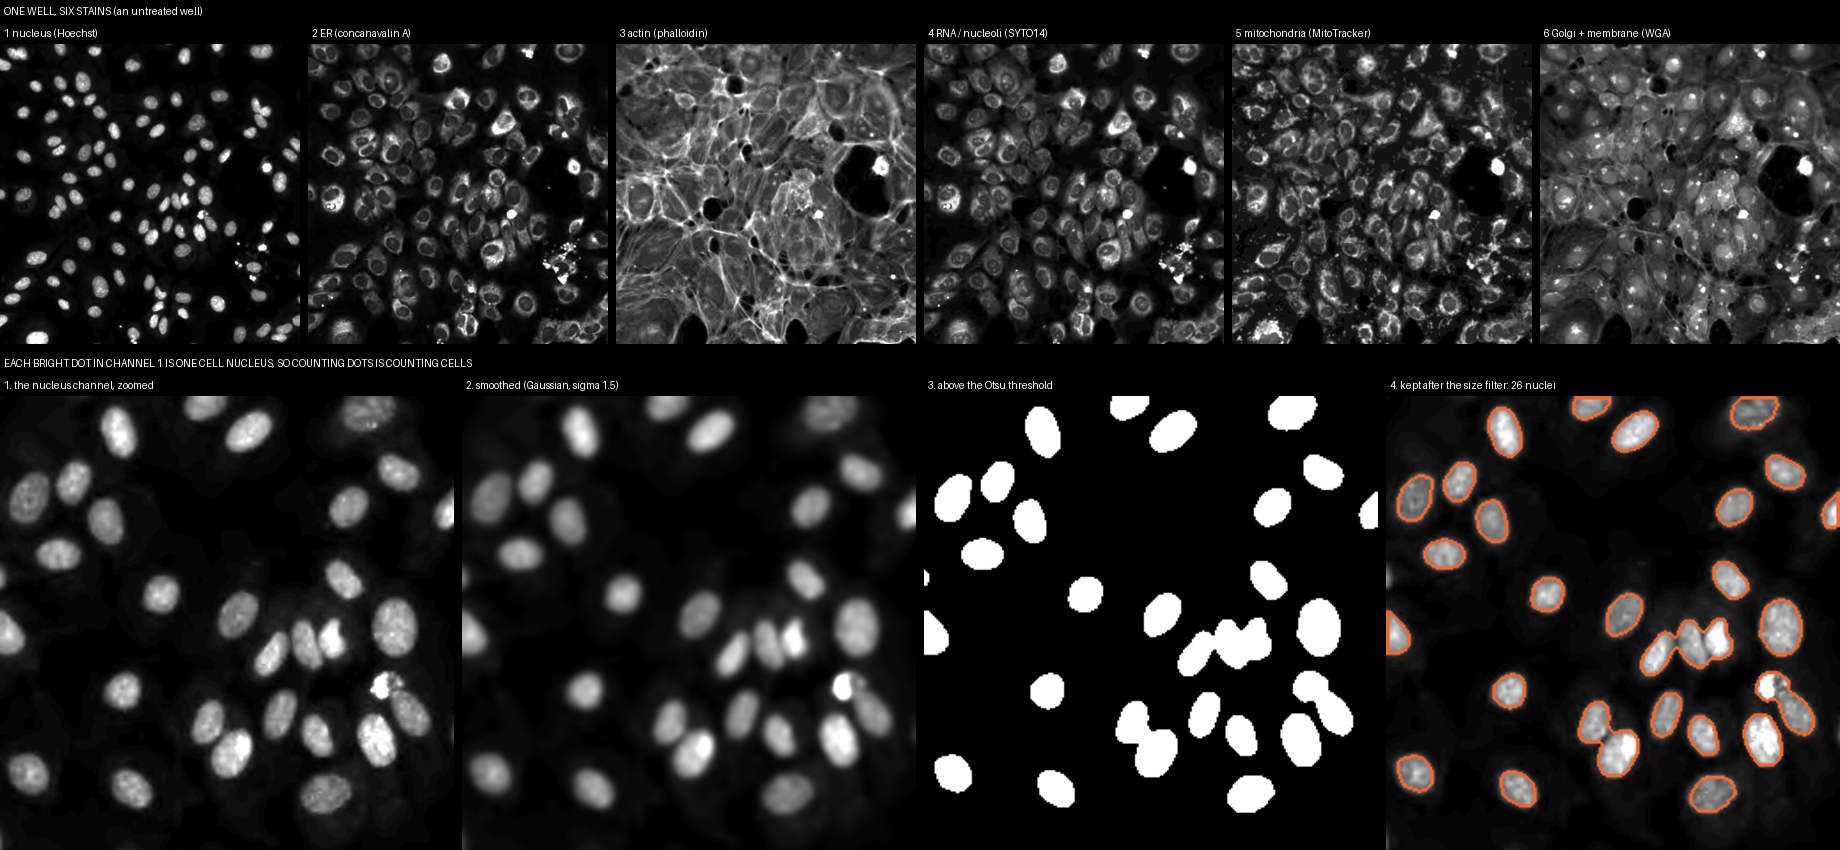
\includegraphics[width=\textwidth]{01_what_is_a_dot.png}
\caption{\textbf{What the data is, and what a cell count counts.} Top: one well in six
channels. Bottom: the nucleus channel, smoothed, thresholded, and filtered by size. Each
bright object in channel~1 is one nucleus, so counting objects is counting cells. The
rendering rule matters beyond this figure: both panels of any comparison are mapped by a
single brightness scale taken from the reference, because contrast-stretching each image
against its own percentiles makes a dim treated well and a bright reference well render
identically.}
\label{fig:dot}
\end{figure}

\section{Predicates, soft labels, and a confound in per-cell features}
\label{sec:confound}

\subsection{Soft predicates}

A predicate is one measurable statement about a group, for example \emph{the
mitochondria are brighter}. It is scored as a probability rather than a class, because
the underlying measurement is continuous and a hard cut discards how far past the
threshold a group sits:
\begin{equation}
p(\text{atom}) \;=\; \sigma\!\left(\frac{s \cdot z - \tau}{T}\right),
\qquad \tau = 2.0,\; T = 0.5,
\end{equation}
with $s=\pm1$ the direction. Both constants were fixed before any model was trained and
never tuned. Cell loss uses the surviving fraction with a cut at $0.6$. Missing
measurements propagate as NaN and are masked, never read as negatives. A goal is a
conjunction of predicates and negated predicates, and its soft label is the product.

\subsection{The confound}

CellProfiler's per-cell features are averages over the objects it can segment, which
are the cells that are still there. A dying cell rounds up and condenses, and therefore
reads \emph{brighter} per unit area in every channel. The consequence is measurable
directly. Against a base rate of 3.5\% of groups showing cell loss, the share of groups
satisfying a per-cell predicate that have \emph{also} lost their cells is:

\begin{center}
\begin{tabular}{lrr}
\toprule
predicate & groups & also lost cells \\
\midrule
brighter DNA staining & 308 & 69\% \\
brighter actin & 107 & 66\% \\
brighter mitochondria & 253 & 64\% \\
smaller nuclei & 211 & 62\% \\
fainter actin & 240 & 56\% \\
bigger nuclei & 212 & 49\% \\
dimmer mitochondria & 81 & 42\% \\
dimmer DNA staining & 57 & 37\% \\
elongated cells & 206 & 16\% \\
\midrule
\textit{base rate} & 13{,}348 & \textit{3.5\%} \\
\bottomrule
\end{tabular}
\end{center}

So \goal{make the mitochondria brighter}, read literally off the features, is
substantially a synonym for \goal{kill the cells}. Any model fitted to that target will
learn the shortcut, and will be right to: it is what the label says.
Figure~\ref{fig:confound} shows the entanglement.

\begin{figure}[t]
\centering
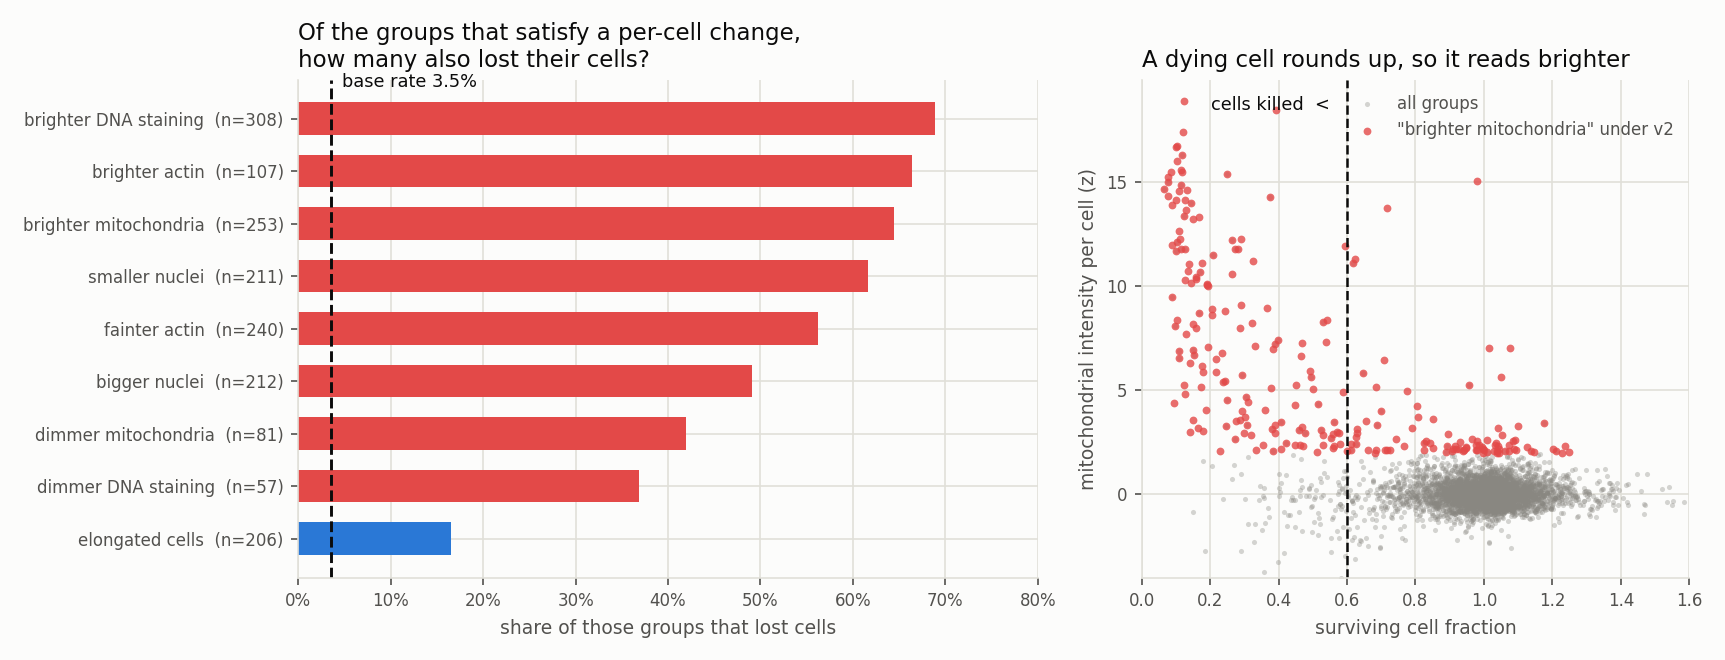
\includegraphics[width=\textwidth]{03_the_definition_problem.png}
\caption{\textbf{The confound.} Left: for each per-cell predicate, the share of
satisfying groups that also lost their cells, against the 3.5\% base rate (dashed).
Right: per-cell mitochondrial intensity against surviving fraction, with the groups
satisfying the literal \goal{brighter mitochondria} predicate highlighted. They are
concentrated where the cells are gone.}
\label{fig:confound}
\end{figure}

\subsection{The redefinition}

We therefore define every per-cell predicate as the conjunction
\begin{equation}
\text{$X$ holds} \;\equiv\; \text{$X$ holds in the measured cells} \;\wedge\; \neg\,\text{cell loss},
\end{equation}
with one exception: if the goal itself asks for fewer cells, its per-cell predicates
keep the literal meaning, since there is nothing left to protect. We write v2 for the
literal definition and v3 for this one. Under v3 the set of goals that nothing in the
archive satisfies grows from 25 to 37, because conjunctions such as \goal{bigger nuclei
and brighter mitochondria} turn out to occur only in dying cells. Both definitions are
implemented and both are reported.

\section{Goals in language}

A goal is an English sentence paired with the formula it stands for. The sentence is all
the model reads; the formula is used only to build the label and to score the answer.
The set contains 259 goals under v3, split four ways.

\begin{center}
\begin{tabular}{llr}
\toprule
split & what is held out & $n$ \\
\midrule
\texttt{train} & nothing & 153 \\
\texttt{para\_test} & the phrasing, for a trained concept & 26 \\
\texttt{comp\_test} & the concept: a conjunction, triple, or negation never trained & 38 \\
\texttt{refuse} & nothing in the archive satisfies it & 37 \\
\texttt{rare\_test} & too few positives in the archive to train on & 5 \\
\bottomrule
\end{tabular}
\end{center}

Five phrasings per predicate were written before any training run; three are trained and
two are held out. Composite goals are generated from templates over pairs and triples of
predicates and over negations. Crucially, \textbf{the refusal set is built by
measurement, not by hand}: every candidate composite is evaluated against the archive,
and those with exactly zero satisfying groups become refusals. This keeps the refusal
task honest, since the impossible goals are impossible as a fact about the library
rather than as a judgement about plausibility.

\section{Model}
\label{sec:model}

Let $e$ be the embedding of the goal sentence under a frozen general-purpose sentence
encoder (\texttt{nli-mpnet-base-v2};~\citealp{reimers2019sbert,song2020mpnet}), $h$ a
chemical representation of the compound, and $z$ the standardised $\log_{10}$ dose. A
shared trunk maps $(e,h)$ to the parameters of a dose response, and the dose is applied
to that curve rather than fed in as another feature:
\begin{equation}
p(\text{goal satisfied} \mid e, h, z) \;=\;
\underbrace{\sigma(b_0 + b_1 z)}_{\text{effect rises}} \cdot
\underbrace{\sigma(c_0 - \operatorname{softplus}(b_3)\, z)}_{\text{survival falls}} .
\label{eq:window}
\end{equation}
The second factor is what makes the output non-monotone, and it is not decoration.
Under v3, 60 of the 80 compounds that ever brighten mitochondria in living cells peak
\emph{below} the top dose, because the top dose kills (Figure~\ref{fig:window}). A
monotone output cannot represent a dose window and will prefer the toxic compound. The
$\operatorname{softplus}$ keeps survival decreasing in dose, so the two factors cannot
exchange roles and fit the window upside down.

\begin{figure}[t]
\centering
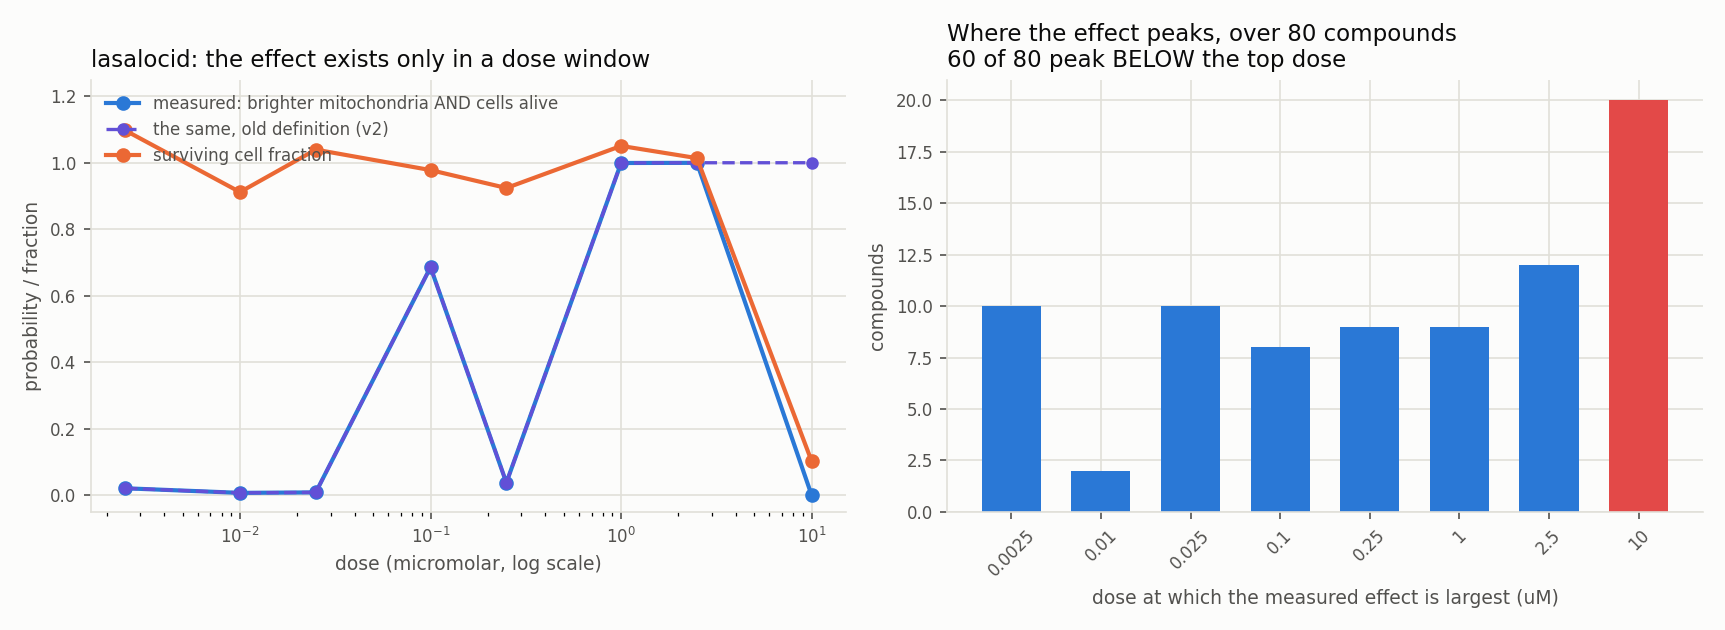
\includegraphics[width=\textwidth]{04_dose_window.png}
\caption{\textbf{Why the output is non-monotone.} Left: one compound's measured
probability of \goal{brighter mitochondria in living cells}, its literal v2 counterpart,
and its surviving fraction, against dose. Right: for the 80 compounds that satisfy the
v3 predicate anywhere, the dose at which the measured effect is largest. Sixty of them
peak below the top dose.}
\label{fig:window}
\end{figure}

The chemical representation is a Morgan count fingerprint~\citep{rogers2010ecfp}
concatenated with MACCS keys and the standardised RDKit~\citep{rdkit} 2D descriptor
block. Each behaviour is sampled as its own task with equal weight, so a common
behaviour such as cell loss cannot drown a rare one by appearing more often. Training
uses cross-entropy against the soft targets, AdamW, and early stopping on held-out
\emph{compounds}. Interference between behaviours was measured rather than assumed: the
cosine between per-behaviour gradients on the shared trunk is about zero with 41--56\%
of pairs negative, yet one joint model beats separate single-behaviour models on unseen
compounds; PCGrad~\citep{yu2020pcgrad}, a mixture of experts, explicit logic heads, a
Hill-shaped output, and an auxiliary embedding loss each changed held-out AUC by at most
$0.01$ and are not used.

\section{Evaluation}

\subsection{Splits}

Compounds are split by Bemis-Murcko scaffold~\citep{bemis1996scaffold} into 70/10/20
train/validation/test, so a test compound shares no ring skeleton with any training
compound. Splitting at random would place salts and close analogues on both sides and
report interpolation~\citep{wallach2018memorization}. No test compound is seen by the
model or by the early-stopping rule, and the refusal threshold is calibrated on the
validation compounds only.

\subsection{Metrics, and two baselines that never read the question}

We report mean AUC over held-out goals, and top-1 hit rate. AUC is the headline because
positives are 1--5\% of groups, so a model that answers ``no'' to everything would post
95\% accuracy.

Every number is reported beside two baselines:

\begin{itemize}\itemsep0.2em
\item \textbf{toxicity-only}: take the model's own prediction for the single instruction
\goal{kill most of the cells} and use that one vector to score \emph{every} goal. It
never reads the question.
\item \textbf{dose-only}: rank by concentration.
\end{itemize}

This is the paper's methodological recommendation, and it costs nothing: both baselines
are free given a trained model.

\subsection{The refusal statistic}

Refusal is scored over the 37 impossible goals against the 64 achievable held-out goals,
using the model's confidence for the goal. The confidence is the \emph{mean of the
top-10 scores}, not the maximum. A maximum is an extreme-value statistic: it grows with
the number of groups in the pool, so a threshold learned on one pool does not transfer
to a larger one, and a single lucky group suffices to answer a goal nothing satisfies.
Measured here, going from 1{,}256 to 2{,}670 groups, the median maximum for impossible
goals rose from $0.038$ to $0.083$ while the achievable ones did not move. Refusal AUC
is $0.85$ with the top-10 mean and $0.79$ with the maximum. Ten is the length of the
shortlist the system displays, fixed in advance rather than tuned.

\subsection{Screening cost}
\label{sec:screening}

AUC does not state a cost. We therefore also report, for each held-out goal, whether the
top $k$ (compound, dose) pairs contain at least one that actually satisfies it, for
budgets corresponding to plate formats, and the number of wells opened before the first
real hit.

\section{Results}
\label{sec:results}

\subsection{The headline, and the baseline beside it}

Five-seed ensemble, unseen-scaffold compounds:

\begin{center}
\begin{tabular}{lcccc}
\toprule
 & \multicolumn{2}{c}{\textbf{v3} (``and the cells survive'')} & \multicolumn{2}{c}{v2 (literal)} \\
\cmidrule(lr){2-3}\cmidrule(lr){4-5}
 & unseen phrasing & unseen concept & unseen phrasing & unseen concept \\
\midrule
model                  & \textbf{0.799} & \textbf{0.861} & 0.842 & 0.873 \\
toxicity-only baseline & 0.696 & 0.789 & 0.833 & 0.855 \\
dose-only baseline     & 0.722 & 0.761 & 0.758 & 0.775 \\
\midrule
margin over toxicity   & \textbf{+0.104} & \textbf{+0.072} & +0.010 & +0.018 \\
\bottomrule
\end{tabular}
\end{center}

The v2 column is the result of this work had the confound not been found: a better
headline and almost nothing behind it. The v3 column is lower and roughly ten times
further from the baseline. Figure~\ref{fig:baselines} shows both.

\begin{figure}[t]
\centering
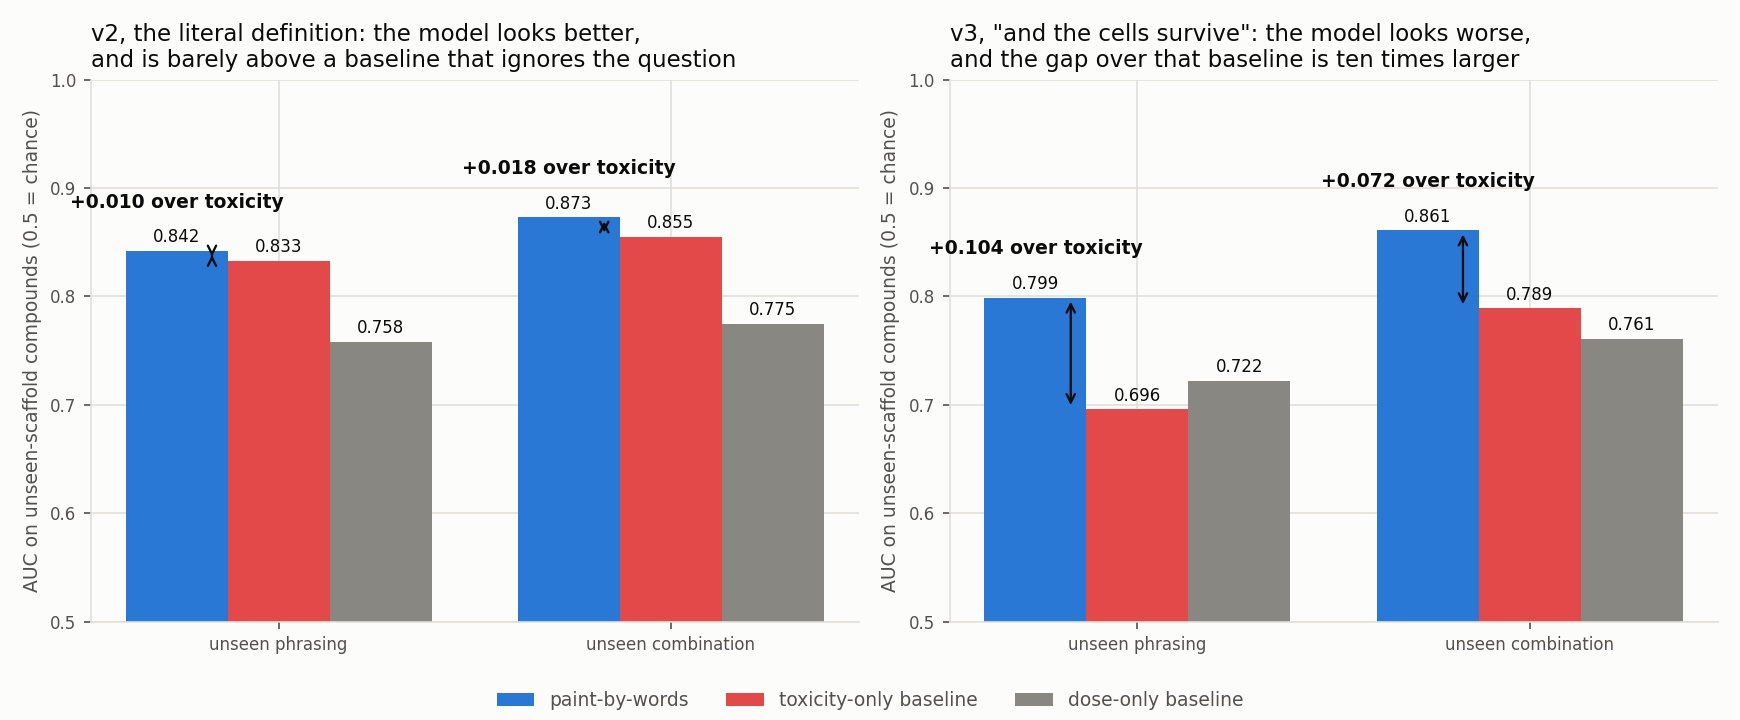
\includegraphics[width=\textwidth]{05_against_the_baselines.png}
\caption{\textbf{The same system under both predicate definitions.} Under the literal
definition the model scores higher and sits almost on top of a baseline that ignores the
question. Under the definition that requires the cells to survive, it scores lower and
the margin is ten times larger. Bars start at $0.5$, which is chance.}
\label{fig:baselines}
\end{figure}

On compounds the model has seen, it reaches $0.929/0.969$, so the bottleneck is
chemistry to phenotype rather than language or capacity.

\subsection{Refusal}

Refusal AUC on unseen compounds is $0.85$ (64 achievable goals against 37 impossible
ones). At the threshold calibrated on validation compounds the system answers 89\% of
the answerable goals and wrongly answers 38\% of the impossible ones. Calibrating the
threshold on \emph{training} compounds instead fails badly: the model fits them closely,
its confidence there is systematically higher than it will ever be on new chemistry, and
the resulting threshold answers only 16\% of answerable goals.

\subsection{What it saves, counted in wells}

\begin{figure}[t]
\centering
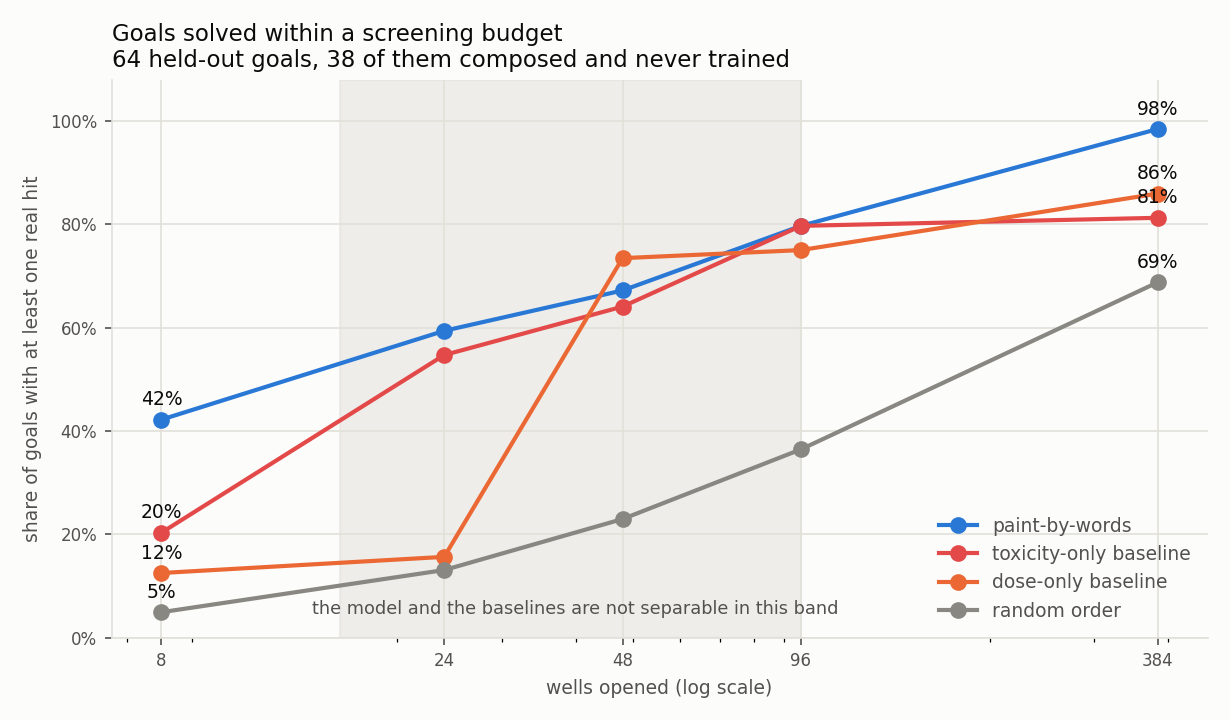
\includegraphics[width=0.92\textwidth]{06_screening_budget.png}
\caption{\textbf{Goals solved within a screening budget.} 64 held-out goals on
unseen-scaffold compounds, 38 of them conjunctions whose concept was never trained. The
model's advantage over the trivial baselines is confined to very small budgets and to
the ceiling; in between, including one budget at which dose-only wins outright, the
curves are not separable.}
\label{fig:screening}
\end{figure}

\begin{center}
\begin{tabular}{lcccc}
\toprule
budget & model & toxicity-only & dose-only & random \\
\midrule
8 wells (one plate row) & \textbf{42\%} & 20\% & 12\% & 5\% \\
24 & 59\% & 55\% & 16\% & 13\% \\
48 & 67\% & 64\% & \textbf{73\%} & 23\% \\
96 (one plate) & 80\% & 80\% & 75\% & 36\% \\
384 & \textbf{98\%} & 81\% & 86\% & 69\% \\
\midrule
median wells to first hit & 12 & 18 & 38 & 267 \\
\bottomrule
\end{tabular}
\end{center}

Read honestly, the reduction from 267 wells to 12 is \emph{not} what the language
channel bought: a baseline that never reads the question reaches 18, and at a budget of
48 wells ranking by dose alone beats the model outright. Goal-specific skill appears in
exactly two places, and both are real:

\begin{itemize}\itemsep0.2em
\item \textbf{At a very small budget.} With eight wells the model solves 42\% of goals
against 20\%; paired over the same goals the difference is $+22\%$, 95\% CI
$[+11\%,+33\%]$, with 15 goals solved only by the model against 1 solved only by the
baseline, McNemar $p=0.0005$. Small budgets are the normal case, since a hypothesis
rarely receives more than a few wells.
\item \textbf{At the ceiling.} With 384 wells the model solves 98\% against 81\%: about
one goal in five is not reachable along the toxicity route at any budget.
\end{itemize}

Between 16 and 96 wells the model and the baselines are not separable (at 16 wells,
$+11\%$, $p=0.12$). We report that null because it bounds the claim.

\subsection{Composition}

Thirty-eight of the 64 held-out goals are conjunctions, triples, or negations whose
concept was never a training target. They are enriched at the same rates as the
single-predicate goals. This is what makes the coverage cheap: a handful of trained
behaviours is composed in language into a much larger space of goals, each answered
without a screen of its own.

\subsection{What fails}

\paragraph{Top-1.} On unseen concepts the toxicity-only baseline picks a correct single
compound more often than the model does ($0.158$ against $0.105$), although the model
orders the library far better ($0.861$ against $0.789$). Ranking skill and single-pick
skill are different, and only the first is established here.

\paragraph{Direction.} The frozen sentence encoder does not encode direction. It places
\goal{push the actin out to the edge} and \goal{pull the actin away from the edge} at
cosine $0.76$, and \goal{make the Golgi smoother} next to \goal{patchy Golgi} at $0.65$.
For such goals the model answers the opposite question confidently, which is the worst
failure mode available to a screening tool. The released system audits every query for
this condition and warns; it does not fix it. Fine-tuning the encoder's last layers
raised top-1 but degraded refusal.

\paragraph{Out-of-scope detection.} Cosine to the nearest trained phrasing cannot
separate a genuine held-out paraphrase ($0.41$--$0.92$) from a deliberately absurd
request ($0.12$--$0.53$); the distributions overlap. The usable guard is the refusal
score, not the encoder.

\section{A vision-language model as a second measuring instrument}
\label{sec:vlm}

The measurement branch reads eight engineered columns. We also tested replacing the
feature extractor entirely with a general-purpose vision-language model, used as a blind
scorer, producing labels for exactly the same formulas, so that the comparison isolates
the instrument.

Two thousand groups were rendered as a treated panel beside a reference panel from the
same plate, six channels each, two native-resolution $256\times256$ crops, with one
brightness scale per channel taken from the reference. Group identifiers were blind. The
model returned seven scores from 0 to 100 with 50 meaning ``no different from the
reference''. Calibration was label-free, $z = (\text{score}-50)/(1.4826\,\text{MAD})$
followed by the same fixed-threshold rule as the measurement branch, so the physical
measurements were never used to calibrate.

Agreement with the measurements, behaviour by behaviour (AUC): cell loss $0.93$,
elongation $0.87$, dimmer DNA $0.81$, dimmer mitochondria $0.75$, fainter actin $0.74$,
brighter actin $0.73$, brighter mitochondria $0.69$, bigger nuclei $0.66$, brighter DNA
$0.59$, smaller nuclei $0.58$. The pattern is interpretable: the model is reliable at
counting and at gross shape, mediocre at ``dimmer'', and weakest at ``brighter'' and at
small size changes, which are exactly the comparisons a human eye also finds hard across
two panels.

\textbf{Trained as a label source, this branch ranks unseen compounds below its own
toxicity-only score} ($-0.02$/$-0.08$ AUC). Doubling the labels from 1{,}000 to 2{,}000
groups gained $+0.04$ and then saturated; the 2{,}000 groups already cover 100\% of the
positives that exist in the archive for these behaviours among training compounds, so
the ceiling is the archive rather than the labelling budget. A single-cell montage view
(24 nucleus-centred tiles per well) was not significantly better than field crops alone
($+0.016$, 95\% CI $[-0.03,+0.06]$); the two views combined were ($+0.036$, 95\% CI
$[+0.011,+0.057]$), at a cost that did not justify scaling.

The practical lesson from this branch is about rendering rather than modelling. In an
earlier round each panel was contrast-stretched against its own percentiles, and the
same model scored at chance on four of eight behaviours, because a dim treated well and
a bright reference well rendered identically. A single shared brightness scale moved
those four behaviours to AUC $0.81$--$1.0$. The failure was in the pipeline.

\section{Limitations}

\textbf{It selects, it does not design.} The system ranks compounds already in the
library at doses already run.

\textbf{Everything here is retrospective.} No prediction has been tested at the bench.

\textbf{``Unseen'' means unseen chemistry under the same measurement conditions.}
Compounds are held out by scaffold, but training and test share plates and staining
batches. In this archive 1{,}661 of 1{,}671 compounds appear in only one of the four
experiments, so holding out an experiment would hold out its compounds too and the two
effects could not be separated. Batch transfer is therefore \emph{unmeasured} here, and
measuring it requires an archive in which the same compounds are run across sources,
such as JUMP cpg0016~\citep{chandrasekaran2023jump,weisbart2024gallery}.

\textbf{The behaviours are eight image features.} ``Brighter mitochondria'' means a
per-cell intensity statistic is high. It is not a claim about mitochondrial biology.

\textbf{One cell type}, and rare goals have very few positives: some held-out goals have
3--10 satisfying groups in the entire archive, where a good AUC is close to a coin flip
with a number attached. The released system reports that support count with every
answer.

\section{A pre-registered prospective test}
\label{sec:prereg}

The single result that would change the status of this work from a retrospective method
to a validated instrument is small and cheap, and we state it in advance so that it
cannot be adjusted afterwards.

\begin{quote}
\textbf{Design.} For each goal, two shortlists of eight (compound, dose) wells are
sealed before any plate is run: one from the model, one from the toxicity-only baseline.
Wells are run blind and scored by the pre-specified predicate.
\textbf{Hypothesis.} The model's shortlist contains a real hit for more goals than the
baseline's.
\textbf{Power.} At the discordance rate measured here (15 goals against 1), 80\% power
requires approximately 30 goals, that is $30 \times 2 \times 8 = 480$ wells, under two
384-well plates.
\textbf{Decision rule.} McNemar's exact test at $\alpha = 0.05$ on the paired outcomes.
\end{quote}

The assumption that carries risk is that the discordance rate holds prospectively. A
prospective run also necessarily introduces a new batch, so it tests batch transfer at
the same time, which the retrospective evaluation could not.

\section{Conclusion}

An experimental archive can be addressed by outcome rather than by treatment, in
ordinary language, returning an intervention and a dose and declining when the library
cannot comply. On a public industrial Cell Painting archive the goal-specific part of
that ability is real but modest: $+0.10$ AUC over a baseline that never reads the
question, a doubled hit rate at an eight-well budget, and access to roughly one goal in
five that general cytotoxicity cannot reach.

The more transferable finding is methodological. Per-cell features computed over
segmented survivors are entangled with cell death strongly enough that the literal
reading of a morphological predicate turns a phenotype model into a toxicity detector
while the headline number improves. The control that detects this is one line of code:
score every goal with the model's own prediction for a single toxicity goal, and report
the difference next to the result. We would not have found our own error without it, and
we suspect the same control is worth running wherever these archives are used.

\section*{Acknowledgements}

This work was carried out independently and received no specific funding, while the
author held a postdoctoral position at the University of Vermont. The data
are RxRx3-core, published by Recursion Pharmaceuticals under its end-user licence; we
thank the authors for releasing it.

\section*{Data and code availability}

The archive is not redistributed. Code, the full instruction set with its splits, the
evaluation protocol including both trivial baselines, and the exact scoring prompt used
for the vision-language branch are available at
\url{https://github.com/drnamlabs-gif/paint-by-words}.

\appendix
\section{Reproducibility}

Predicate thresholds ($\tau = 2.0$, $T = 0.5$, surviving-fraction cut $0.6$) were fixed
before training and never tuned. The scaffold split seed is held constant across model
seeds. Reported numbers are five-seed ensembles. The sentence encoder is frozen. The
vision-language branch used a general-purpose commercial model accessed as an agent with
read access to the rendered panels and to nothing else; the exact prompt is released
verbatim with the code, since its wording measurably changes the scores. Every figure and
table in this paper is regenerated by a single command in the released repository.

\bibliographystyle{plainnat}
\bibliography{refs}

\end{document}
